\section{Pendahuluan}
\subsection{Latar Belakang}
Manajemen bandwidth adalah suatu pendekatan yang digunakan untuk mengatur dan
mengontrol penggunaan bandwidth dalam suatu jaringan komputer. Dalam jaringan yang
sibuk, alokasi bandwidth yang efisien dan adil sangat penting untuk menjaga kinerja jaringan
yang optimal. Salah satu cara untuk mengimplementasikan manajemen bandwidth adalah
dengan menggunakan QoS atau Quality of Service.\\\\
Quality of Service (QoS) adalah konsep yang digunakan dalam jaringan komputer untuk
mengatur dan memberikan prioritas terhadap jenis-jenis data yang berbeda. Dengan
menerapkan QoS, administrator jaringan dapat mengatur penggunaan bandwidth, latency,
jitter, dan keandalan layanan dalam jaringan. QoS memungkinkan pengaturan prioritas,
pembatasan bandwidth, dan penjadwalan yang lebih baik untuk aplikasi atau protokol
tertentu.\\\\
Dalam lingkungan jaringan yang padat, sering kali beberapa pengguna menggunakan aplikasi
atau protokol yang mengkonsumsi bandwidth yang tinggi, seperti video streaming atau file
sharing, sementara pengguna lainnya mungkin hanya perlu menggunakan aplikasi yang
membutuhkan bandwidth yang lebih rendah, seperti browsing web atau email. Tanpa
manajemen bandwidth yang efektif, pengguna dengan aplikasi berat bisa mendominasi
sebagian besar bandwidth, menyebabkan kualitas layanan yang buruk bagi pengguna lain.
Simple Queue adalah salah satu metode manajemen bandwidth yang umum digunakan dalam
router atau perangkat jaringan untuk mengatasi masalah ini.\\\\
Dalam Simple Queue, bandwidth diatur dengan membuat aturan atau kebijakan yang
mendefinisikan sejumlah parameter, seperti kapasitas maksimum bandwidth yang dapat
digunakan oleh pengguna, prioritas, dan pembatasan lainnya. Setiap paket data yang
melewati router akan dicek dan diberi label sesuai dengan aturan tersebut, dan kemudian akan
dikirim atau ditunda sesuai dengan prioritas dan alokasi bandwidth yang ditentukan. Dengan
menggunakan Simple Queue, administrator jaringan dapat memastikan bahwa penggunaan
bandwidth dijaga secara adil dan efisien. Pengguna dengan kebutuhan bandwidth yang tinggi
dapat diberikan alokasi yang lebih besar, sementara pengguna dengan kebutuhan yang lebih rendah tidak akan terpengaruh oleh penggunaan yang berlebihan. Hal ini membantu
memastikan kualitas layanan yang lebih baik bagi seluruh pengguna dalam jaringan. Selain
itu, Simple Queue juga memungkinkan administrator jaringan untuk memprioritaskan jenis
lalu lintas tertentu, misalnya memberikan prioritas lebih tinggi untuk aplikasi bisnis daripada
aplikasi hiburan. Dengan demikian, manajemen bandwidth dengan Simple Queue dapat
membantu meningkatkan efisiensi penggunaan bandwidth, mengoptimalkan kinerja jaringan,
dan menghindari situasi di mana penggunaan bandwidth yang tidak adil atau berlebihan
mengganggu pengalaman pengguna lainnya.

\subsection{Maksud dan Tujuan}
Mengetahui cara melimitasi dan memanagemen bandwith untuk suatu jaringan yang banyak pengguna.

\subsection{Hasil yang diharapkan}
Dapat memahami pengonfigurasian terkait Bandwith menggunakan Qos (Simple Queue)

%===========================================================%
\section{Tugas Pendahuluan}
\begin{enumerate}
	\item Halo
\end{enumerate}

\begin{center}
	\colorbox{cyan!30}{\parbox{0.8\linewidth}{\textbf{Opsional:} Pelajari Git dan Github. Anda dapat memulai pembelajaran dari sumber berikut ini: \\ \href{https://github.com}{GitHub - https://github.com} \\ \href{https://git-scm.com/doc}{Git -https://git-scm.com/doc}}}
\end{center}

%===========================================================%
\section{Alat dan Bahan}
\begin{itemize}[label=$\bullet$, itemsep=-1pt, leftmargin=*]
	\item 1 RouterOS mikrotik
	\item 2 Laptop
	\item Kabel LAN
	\item Software Winbox
\end{itemize}

%===========================================================%
\section{Jangka Waktu Pelaksanaan}
Pemahaman dan konfigurasi 1 jam.

%===========================================================%
\section{Penjelasan dan Tahapan Konfigurasi}

%======================PERCOBAAN 1==========================%
\subsection{Percobaan 1}
\begin{center}
    \textbf{Konfigurasi Router 1}
    \begin{enumerate}
        \item Buka WinBox
        \begin{figure}[H]
			\centering
			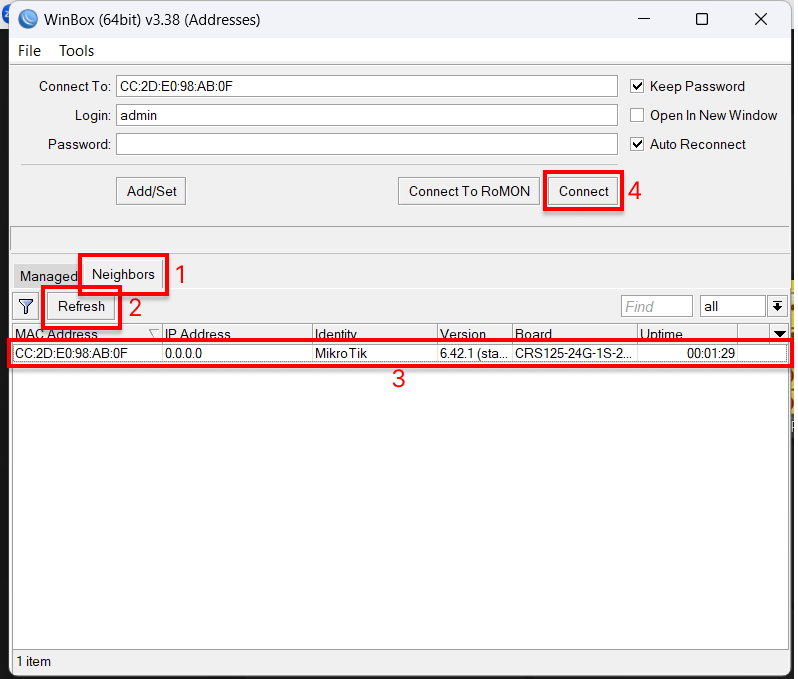
\includegraphics[width=0.8\linewidth]{P3/img/per1/pc1/Step 1.png}
			\caption{Step 1}
			\label{fig:Step 1(Per.1 PC1)}
		\end{figure}
        \item 
    \end{enumerate}

    \textbf{Konfigurasi Router 2}
    \begin{enumerate}
        \item Buka WinBox
        \begin{figure}[H]
			\centering
			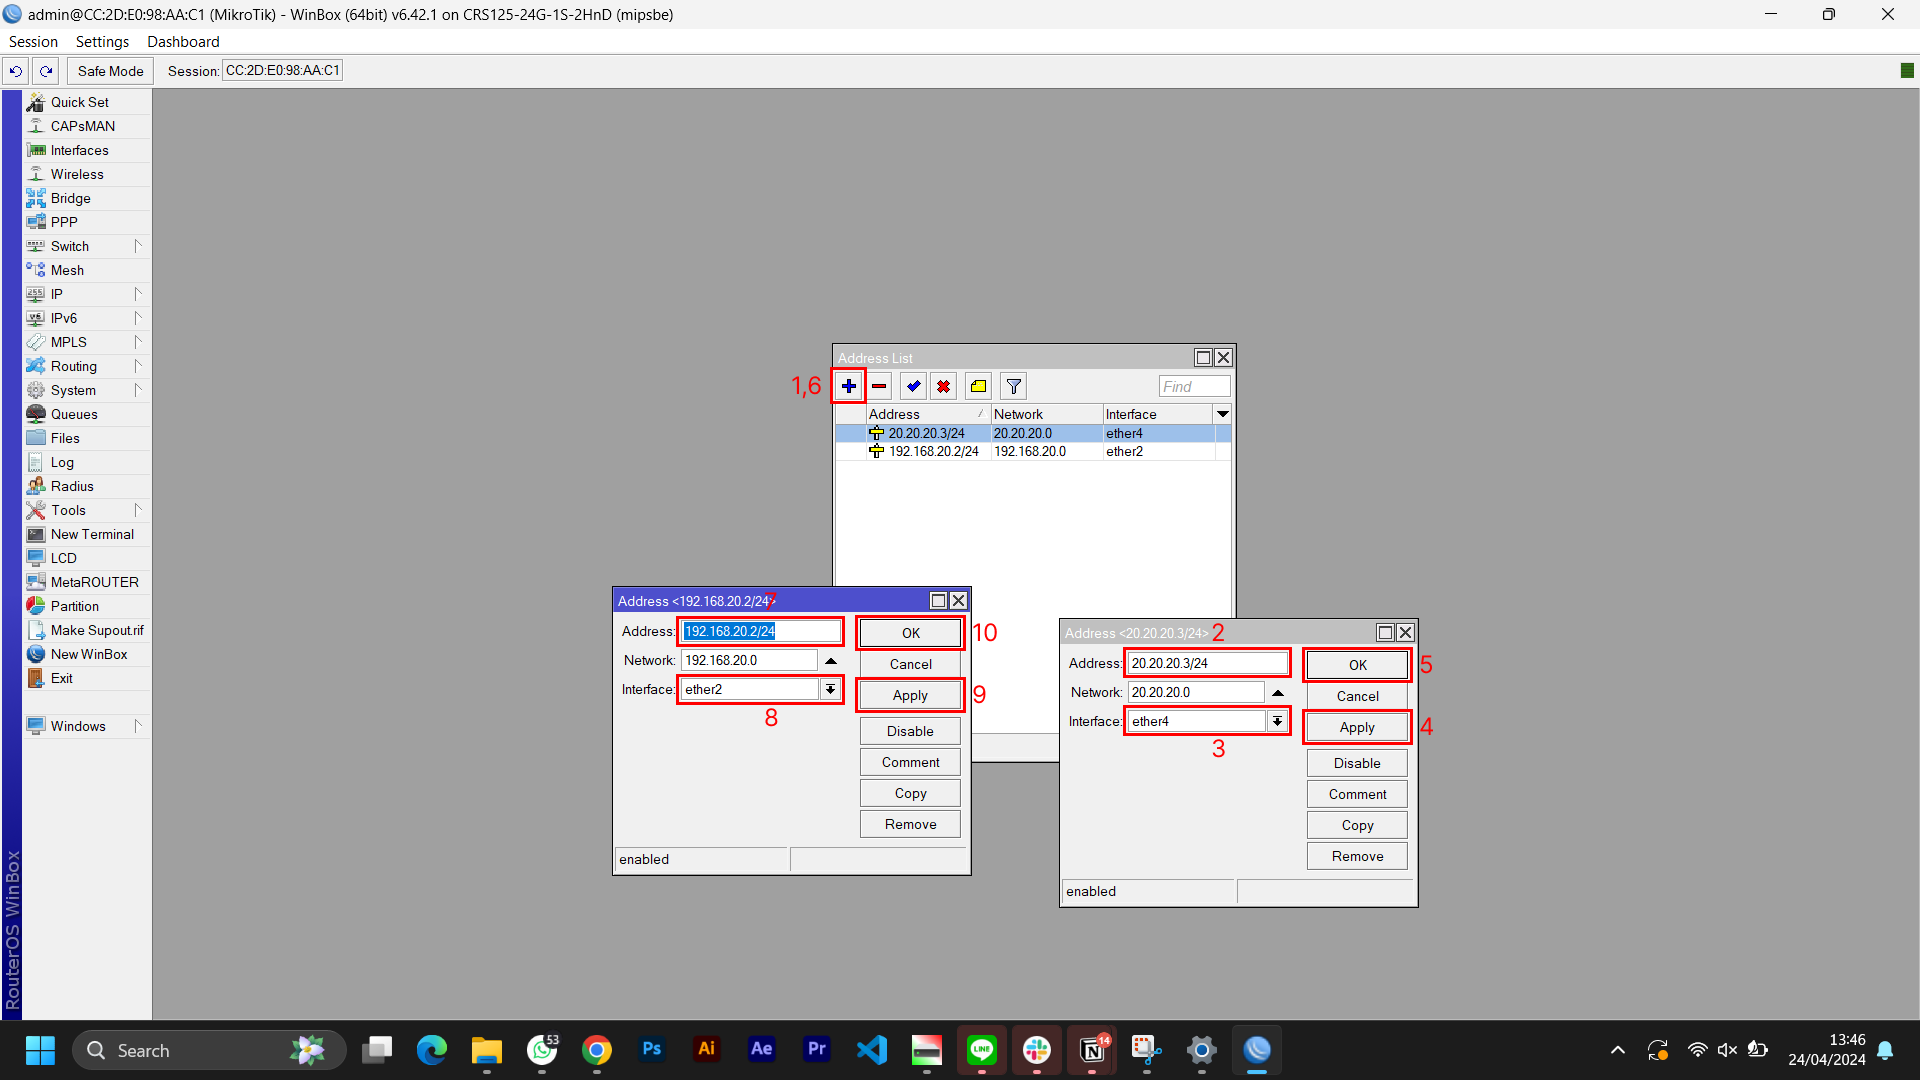
\includegraphics[width=0.8\linewidth]{P3/img/per1/pc2/Step 2.png}
			\caption{Step 2}
			\label{fig:Step 2(Per.1 PC2)}
		\end{figure}
        \item 
    \end{enumerate}

    \textbf{Pengujian Konfigurasi}
    \begin{enumerate}
        \item Lakukan tes ping
        \begin{figure}[H]
			\centering
			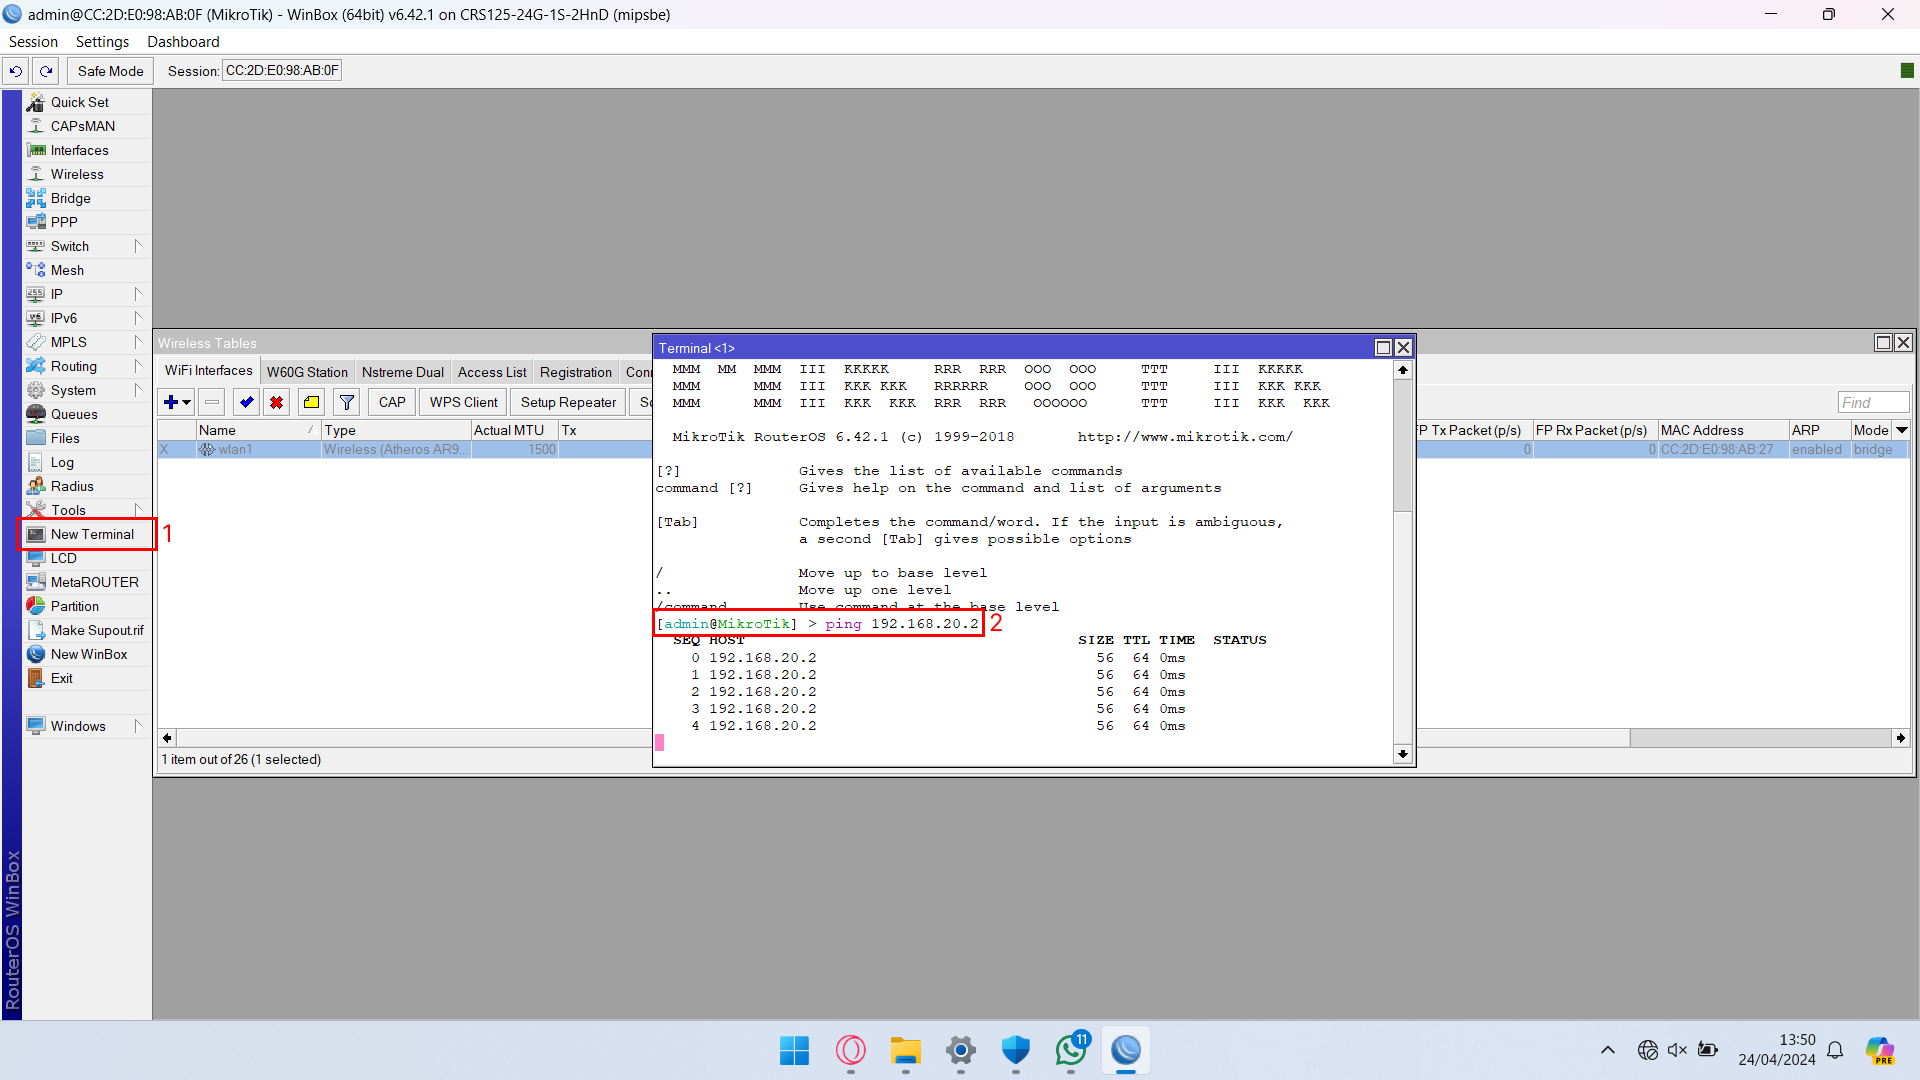
\includegraphics[width=0.8\linewidth]{P3/img/per1/pc1/Step 4.png}
			\caption{Step 1}
			\label{fig:Ping Step 1(Per.1 PC1)}
		\end{figure}
        \item 
    \end{enumerate}
\end{center}

%======================PERCOBAAN 2==========================%
\subsection{Percobaan 2}
\begin{center}
    \textbf{Konfigurasi Router 1}
    \begin{enumerate}
        \item Buka WinBox
        \begin{figure}[H]
			\centering
			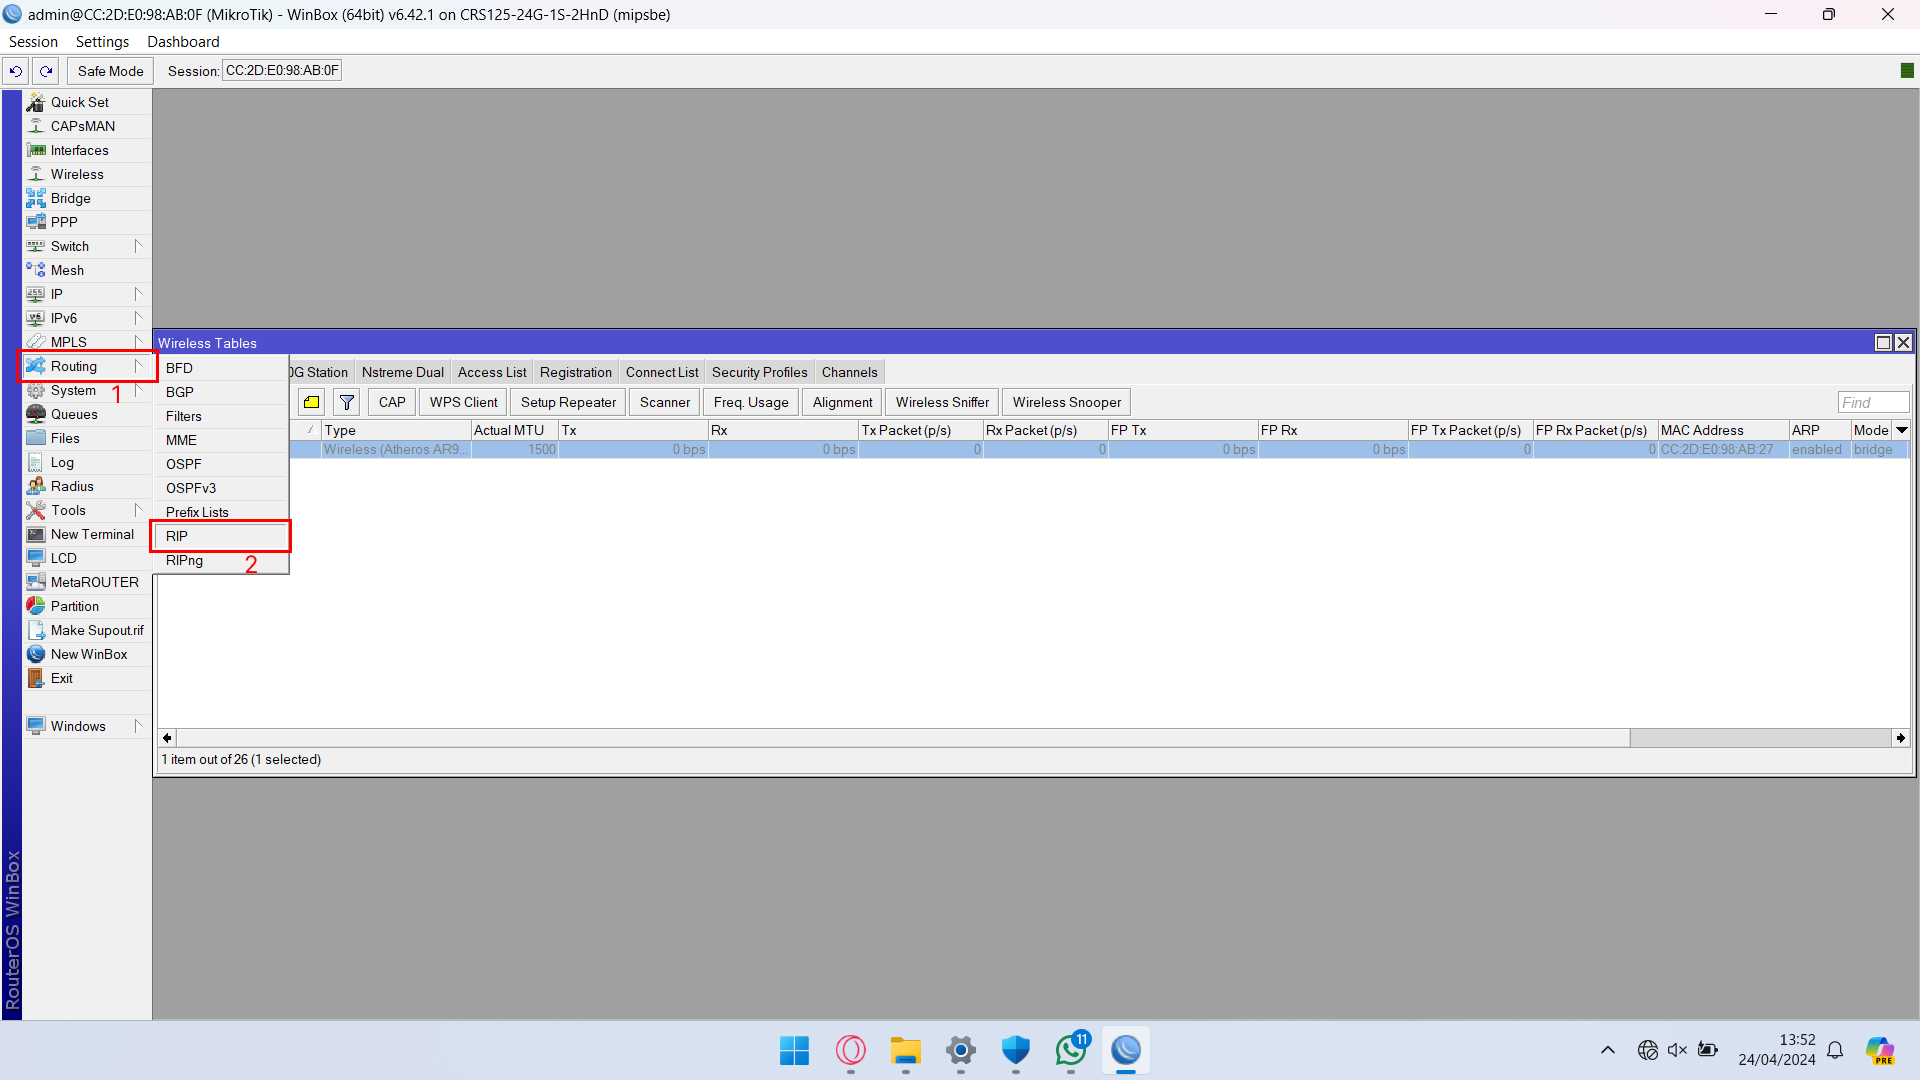
\includegraphics[width=0.8\linewidth]{P3/img/per2/pc1/Step 3.1.png}
			\caption{Step 3.1}
			\label{fig:Step 3.1(Per.2 PC1)}
		\end{figure}
        \item 
    \end{enumerate}

    \textbf{Konfigurasi Router 2}
    \begin{enumerate}
        \item Buka WinBox
        \begin{figure}[H]
			\centering
			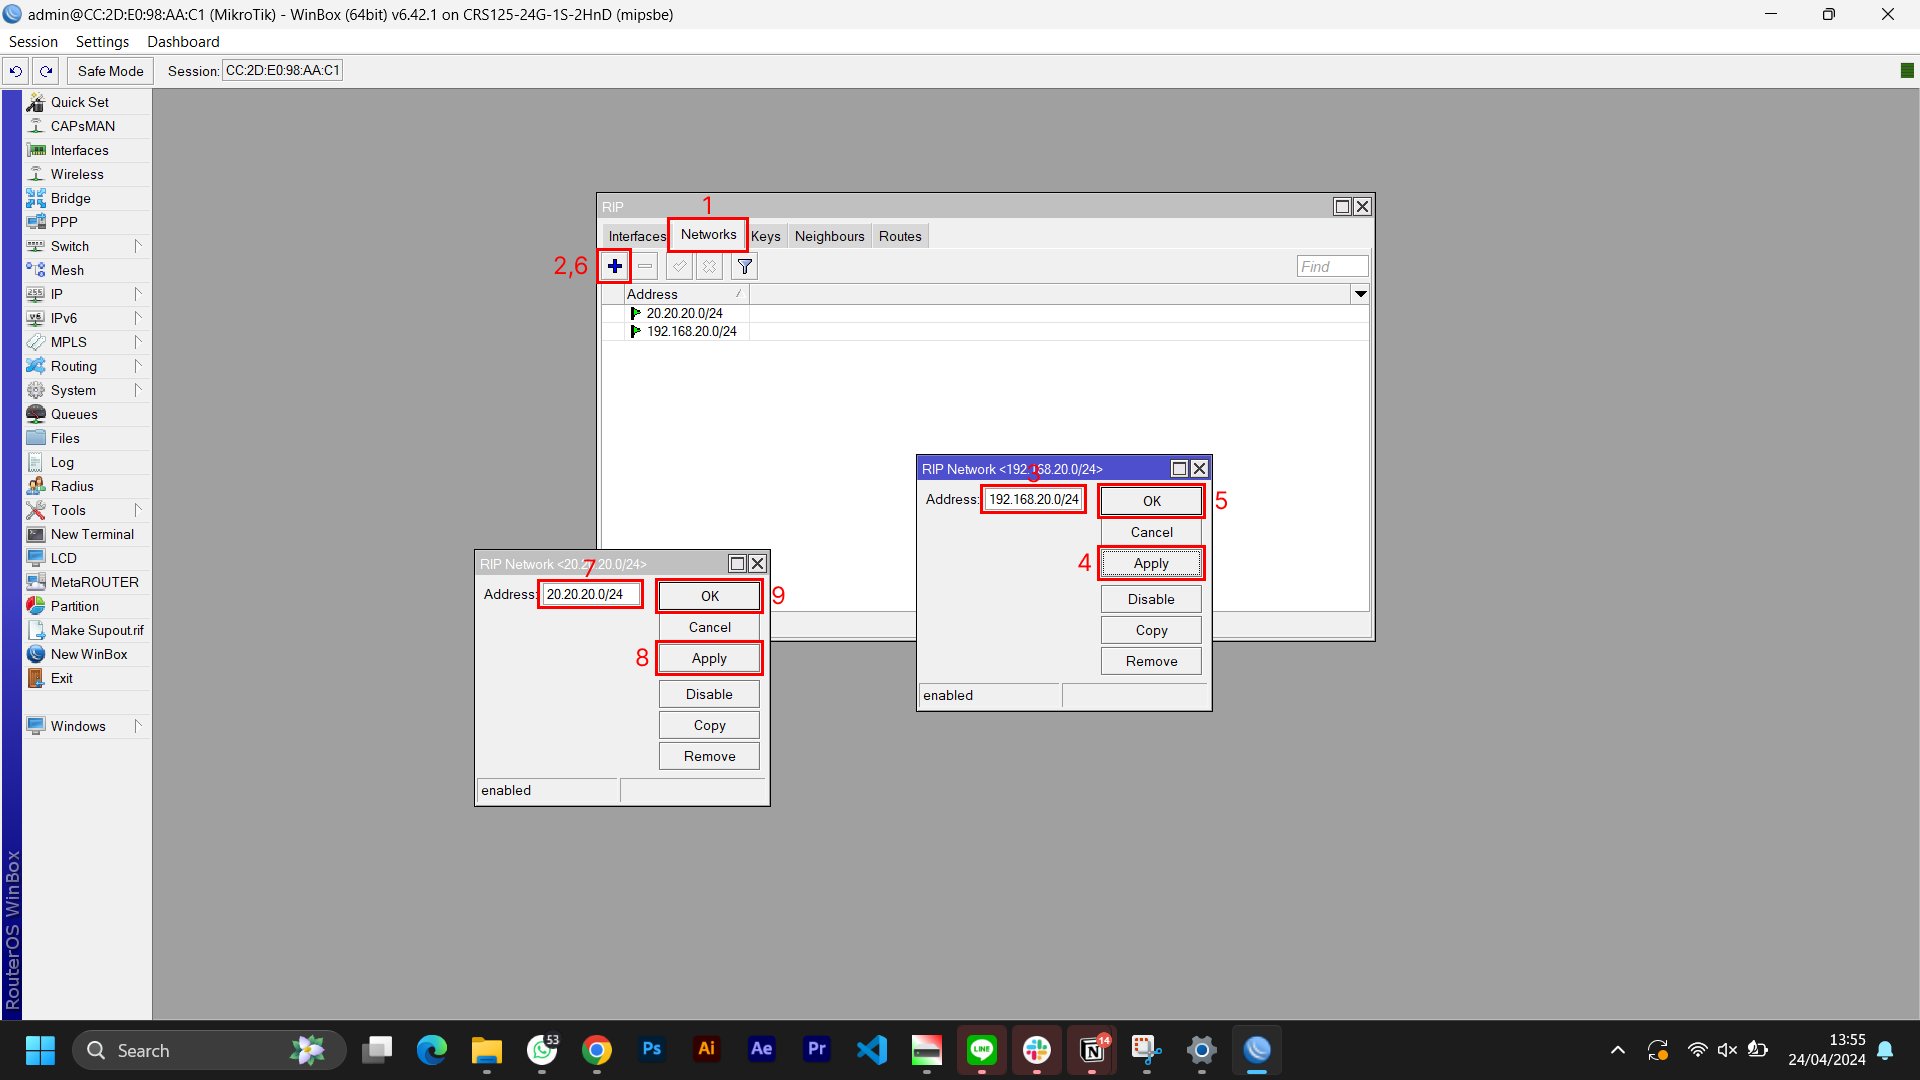
\includegraphics[width=0.8\linewidth]{P3/img/per2/pc2/Step 4.png}
			\caption{Step 4}
			\label{fig:Step 4(Per.2 PC2)}
		\end{figure}
        \item 
    \end{enumerate}

    \textbf{Pengujian Konfigurasi}
    \begin{enumerate}
        \item Lakukan tes ping
        \begin{figure}[H]
			\centering
			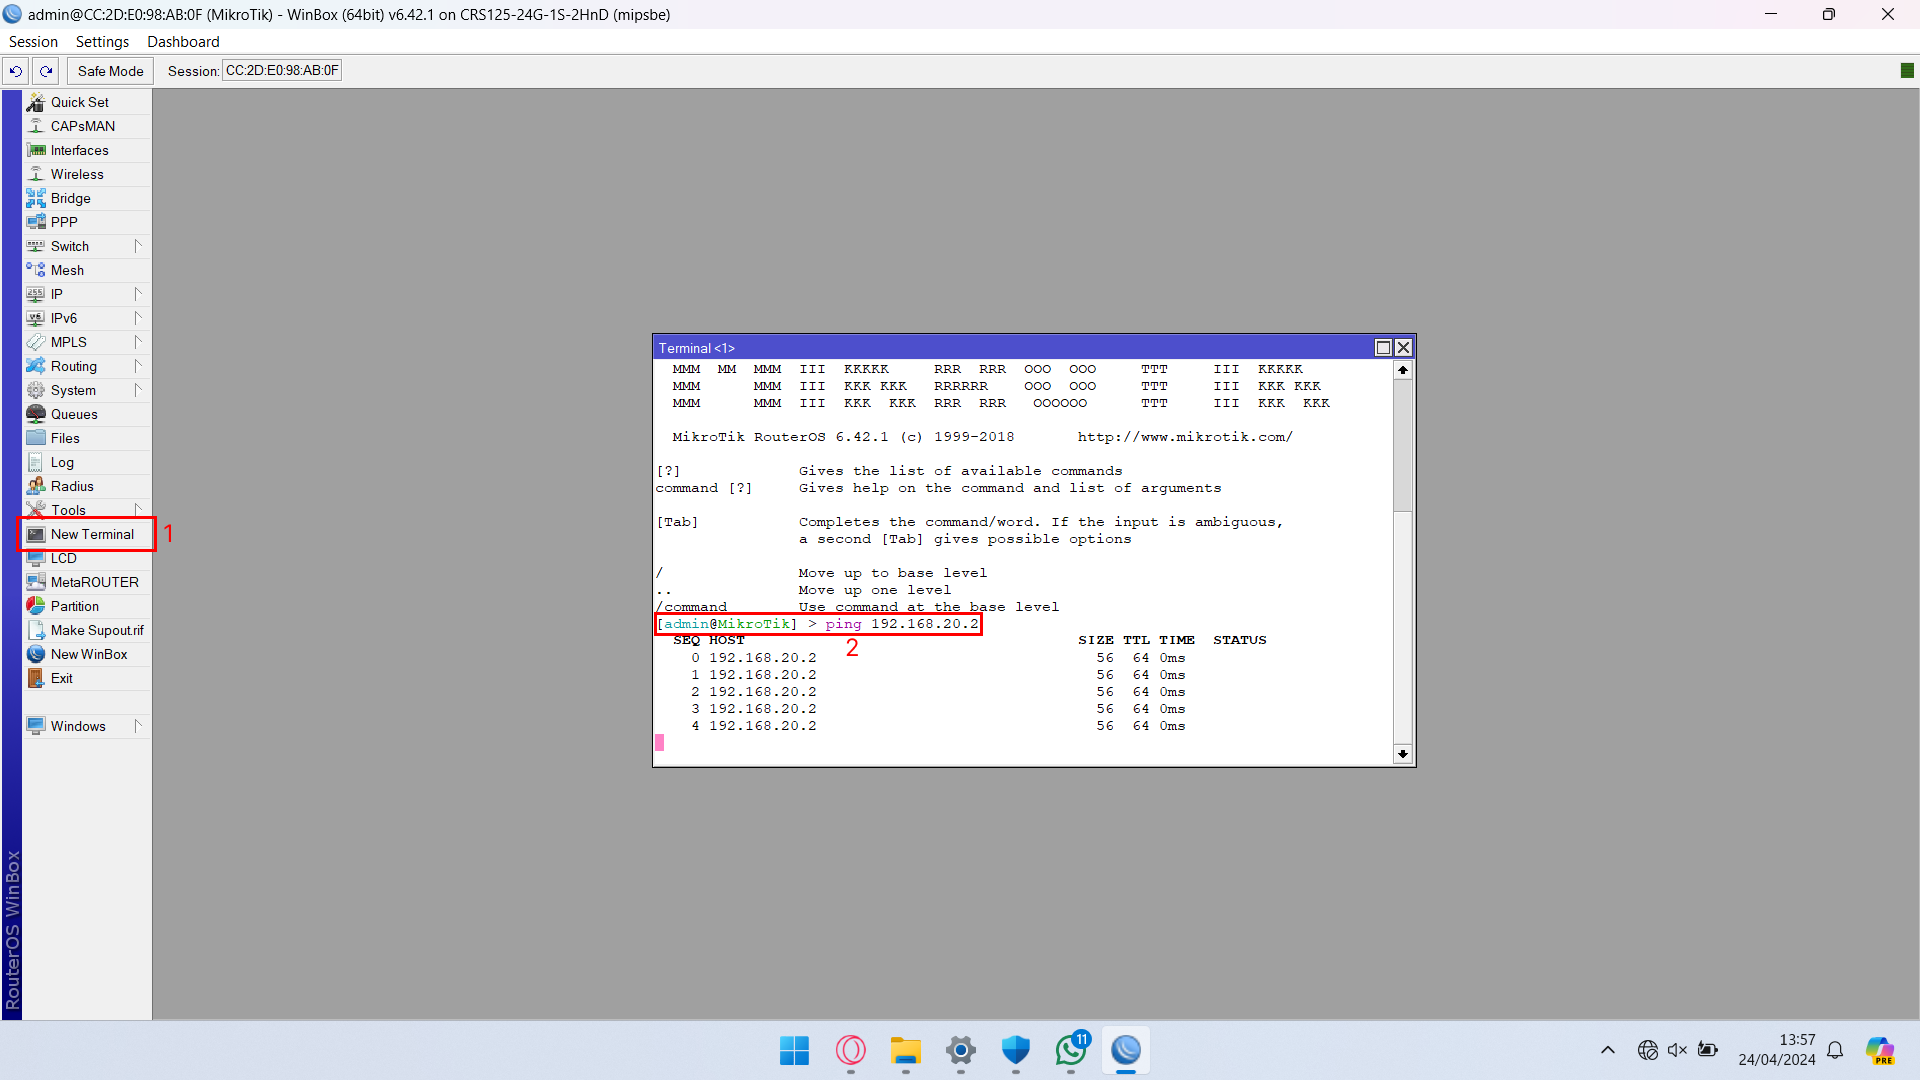
\includegraphics[width=0.8\linewidth]{P3/img/per2/pc1/Step 6.png}
			\caption{Step 1}
			\label{fig:Ping Step 1(Per.1 PC1)}
		\end{figure}
        \item 
    \end{enumerate}
\end{center}

%===========================================================%
\section{Hasil yang didapat}
Memahami dan mengkonfigurasi routing dinamis RIP dengan tepat.

%===========================================================%
\section{Kesimpulan}
Dalam mengkonfigurasi routing RIP, diperlukan pemahaman dasar mengenai setting IP Address dan Subnetting, dan juga diperlukan ketelitian dan fokus agar berhasil
